\documentclass[frenchb]{article}
\usepackage[T1]{fontenc}
\usepackage[utf8]{inputenc}
%Pour utilisation sous unix
%\usepackage[utf8]{inputenc}
%\usepackage[utf8x]{inputenc}
\usepackage{a4wide}
\usepackage{graphicx}
\usepackage{amssymb}
\usepackage{color}
\usepackage{babel}

\begin{document}

\begin{figure}[t]
\centering

\includegraphics[width=5cm]{inp_n7.png}
\end{figure}

\title{\vspace{4cm} \textbf{Manuel du module compression/decompression de fichier texte avec codage de Huffman sous Ada}}
\author{MOUTAHIR Jed\\AIMI Mathis }
\date{\vspace{7cm} Département Sciences du Numérique - Première année \\
2021-2022 }

\maketitle

\newpage
\tableofcontents
%\listoffigures

\newpage
\section{Mise en place du module}
Ce module permet de compresser/décompresser un fichier texte avec le codage de Huffman. Commencez par décompresser le fichier sources.tar.gz dans le répertoire de votre choix. Si les exécutables ne sont pas présents, compiler (par exemple avec GNAT Studio) les fichiers $compression.adb$ et $decompression.adb$.

\section{Compression}
	Pour compresser un fichier entrez la commande : $./compresser \ fichier\_texte.txt$\\
	Voici ce que vous devez obtenir :
	\begin{figure}[ht!]
		\centering
		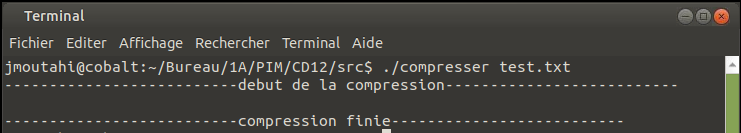
\includegraphics[scale=0.7]{compression.png} 
	\end{figure}
		
	Pour afficher l'arbre de Huffman lors de la compression du fichier entrez la commande : $./compresser \ -b \ fichier\_texte.txt$\\
	Voici ce que vous devez obtenir :
	\begin{figure}[ht!]
		\centering
		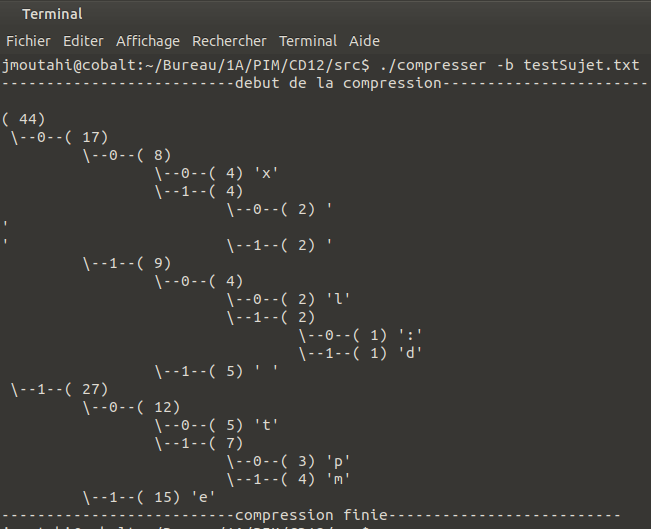
\includegraphics[scale=0.7]{compressionBavarde.png} 
	\end{figure}


\newpage
\section{Décompression}
Pour décompresser un fichier entrez la commande : $./decompresser \ fichier\_texte.txt.hff$\\
Voici ce que vous devez obtenir :
	\begin{figure}[ht!]
		\centering
		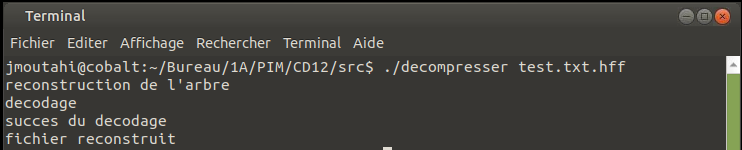
\includegraphics[scale=0.7]{decompression.png} 
	\end{figure}


\end{document} 